\documentclass[12pt,letterpaper]{article}
\usepackage{fullpage}
\usepackage[top=1.5cm, bottom=3.5cm, left=2.2cm, right=2.2cm]{geometry}
\usepackage{amsmath,amsthm,amsfonts,amssymb,amscd, esint}
\usepackage{lastpage}
\usepackage{enumerate}
\usepackage{fancyhdr}
\usepackage{mathrsfs}
\usepackage{graphicx}
\usepackage{listings}
\usepackage{hyperref}
\usepackage[english]{babel}
\usepackage{lipsum}
\usepackage[table,xcdraw]{xcolor}
\usepackage{enumitem}
\usepackage{float}
\usepackage{chemfig}
\usepackage{yfonts}
\usepackage{tikz}
\usepackage{wrapfig}
\usepackage{url}
\usepackage{natbib}
\usepackage[normalem]{ulem}
\usepackage{multicol}
\useunder{\uline}{\ul}{}


%%%%%%%%%%%%%%% CODELISTINGS %%%%%%%%%%%%%%%%
\usepackage{listings}
\definecolor{codegreen}{rgb}{0,0.6,0}
\definecolor{codegray}{rgb}{0.5,0.5,0.5}
\definecolor{codepurple}{rgb}{0.58,0,0.82}
\definecolor{backcolour}{rgb}{0.95,0.95,0.92}

\lstdefinestyle{mystyle}{
    backgroundcolor=\color{backcolour},   
    commentstyle=\color{codegreen},
    keywordstyle=\color{magenta},
    numberstyle=\tiny\color{codegray},
    stringstyle=\color{codepurple},
    basicstyle=\ttfamily\footnotesize,
    breakatwhitespace=false,         
    breaklines=true,                 
    captionpos=t,                    
    keepspaces=true,                 
    numbers=left,                    
    numbersep=5pt,                  
    showspaces=false,                
    showstringspaces=false,
    showtabs=false,                  
    tabsize=2
}

\lstset{style=mystyle}

%%%%%%%%%%%%%%%%%%%%%%%%%%%%%%%%%%%%%%% 




\newtheorem{definition}{Definition}
\newtheorem{observation}{Observation}
\newtheorem{reflection}{Reflection}
\newtheorem{PyPackage}{Package}
\newtheorem{book}{Book}

\newcommand{\HRule}[1]{\rule{\linewidth}{#1}}
\setcounter{tocdepth}{5}
\setcounter{secnumdepth}{5}

\setlength{\parindent}{0.0in}
\setlength{\parskip}{0.05in}

% Edit these as appropriate
\newcommand\course{}
\newcommand\subject{Final Degree Project}
\newcommand\degree{Bachelor's Degree in Physics}
\newcommand\documenttitle{Notes: Quantum State Exclusion - Temporal Name -}
\newcommand\NetIDb{Universitat Autònoma de Barcelona}


\begin{document}
\title{\vspace{4cm} \normalsize 
		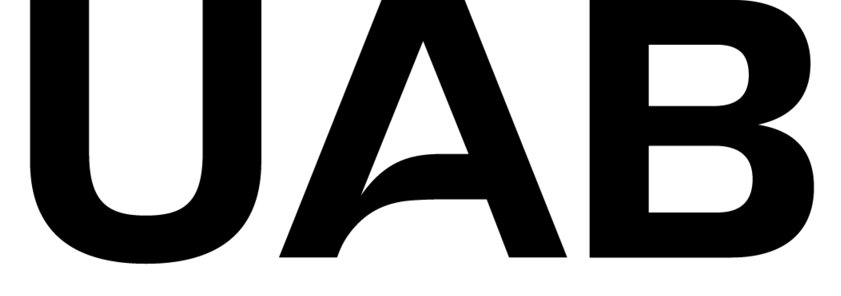
\includegraphics[width = 0.25\textwidth]{GeneralSources/UABLogo.png}\\ [0.5cm]
		\textsc{\NetIDb}\\ [2.0cm]
		\HRule{0.5pt} \\
		\LARGE \textbf{\uppercase{\documenttitle}}
		\HRule{2pt} \\ [1.5cm]
		\normalsize \begin{tabular}{rcl}  % Create a right-left column alignment
        \textsc{Author} & : & \textsc{Sergio Castañeiras Morales} \\
        \textsc{Supervisor} & : & \textsc{Ramón Muñoz Tapia} \\
        \textsc{Co-Supervisor} & : & \textsc{Santiago Llorens Fernández}
    \end{tabular}
    \normalsize \vspace*{5\baselineskip}
		}

\date{2024-2025}

\author{\large \textsc{\subject} \\ \textsc{\degree}}



\begin{titlepage}
\clearpage\maketitle
\thispagestyle{empty}
\end{titlepage}


\newpage
\pagestyle{fancyplain}
\headheight 35pt
\lhead{\NetIDb}    
\rhead{\subject}
\cfoot{}
\rfoot{\small\thepage}
\headsep 1.5em

%%%%%%%%%%%%%%%%%%%%%%%%%%%%%%%%%%%%%%%%%%
%%%%%%%%%%%%%%%%% DEFINITIONS %%%%%%%%%%%%%%%%%
%%%%%%%%%%%%%%%%%%%%%%%%%%%%%%%%%%%%%%%%%%

\begin{multicols}{2}
[
\section{Definitions}
]
\begin{definition}
\textbf{Completely positive map}: "Let $ A $ and $ B $ be C*-algebras. A linear map $ \phi: A \to B $ is called a \textit{positive map} if $ \phi $ maps positive elements to positive elements:
\begin{align}
a \geq 0 \implies \phi(a) \geq 0.
\end{align}

Any linear map $ \phi: A \to B $ induces another map
\begin{align}
\mathrm{id} \otimes \phi : \mathbb{C}^{k \times k} \otimes A \to \mathbb{C}^{k \times k} \otimes B
\end{align}
in a natural way. If $ \mathbb{C}^{k \times k} \otimes A $ is identified with the C*-algebra $ A^{k \times k} $ of $ k \times k $-matrices with entries in $ A $, then $ \mathrm{id} \otimes \phi $ acts as
\begin{align}
\begin{pmatrix}
a_{11} & \cdots & a_{1k} \\
\vdots & \ddots & \vdots \\
a_{k1} & \cdots & a_{kk}
\end{pmatrix}
\mapsto
\begin{pmatrix}
\phi(a_{11}) & \cdots & \phi(a_{1k}) \\
\vdots & \ddots & \vdots \\
\phi(a_{k1}) & \cdots & \phi(a_{kk})
\end{pmatrix}.
\end{align}

The map $ \phi $ is called \textit{k-positive} if $ \mathrm{id}_{\mathbb{C}^{k \times k}} \otimes \phi $ is a positive map, and \textit{completely positive} if $ \phi $ is $ k $-positive for all $ k $."\cite{completely_positive_map_Wikipedia}
\end{definition}
\begin{definition}\textbf{Kraus operator: } 
\end{definition}

\begin{definition}\label{innerProductDefinition}
\textbf{Inner product}: Given a vector space $A$ and a field $F$ we define the an inner product $\langle \cdot , \cdot \rangle$ as $\langle \cdot , \cdot \rangle:A\times A\rightarrow F$ that satisfies the following properties. Given $x,y,z\in A$ and $\lambda,\mu\in F$:
\begin{enumerate}
\item Conjugate symmetry: $\langle x,y\rangle=(\langle y,x\rangle)^*$.
\item Linearity: $\langle \lambda x+\mu y, z\rangle=\lambda\langle  x, z\rangle+\mu\langle  y, z\rangle$
\item Positive-definiteness: $\langle x,x\rangle>0$ if $x\neq0$
\end{enumerate}
\end{definition}

\begin{definition}
\textbf{Inner product space}: Given a vector space $A$ and a field $F$ we define the  inner product space as the duple $(A,\langle \cdot , \cdot \rangle)$ such that  $\langle \cdot , \cdot \rangle:A\times A\rightarrow F$ is an inner product.
\end{definition}

\begin{definition}
\textbf{Gram matrix}: Given a vector space $A$, a field $F$ , a set of vectors $\{v_i\}_{i=0}^n\subset A$ and an inner product space such that  $\langle \cdot , \cdot \rangle:A\times A\rightarrow F$  the Gram matrix $G$ is defined as the matrix $G\in F^{n\times n}$ whose entries are $g_{i,j}=\langle v_i,v_j\rangle$ i.e,
\begin{align}
G=\begin{pmatrix}
\langle v_1,v_1\rangle & \hdots & \langle v_1,v_n\rangle\\
\vdots & \ddots & \vdots\\
\langle v_n,v_1\rangle & \hdots & \langle v_n,v_n\rangle
\end{pmatrix}.
\end{align}
Due to the first property of the inner product definition \ref{innerProductDefinition} it is immediate that $G^\dagger =G$ in other word G is hemitian (trivial proof).
\end{definition}

\end{multicols}
\newpage

%%%%%%%%%%%%%%%%%%%%%%%%%%%%%%%%%%%%%%%%%%
%%%%%%%%%%%%%%%% BIBLIOGRAPHY %%%%%%%%%%%%%%%%%
%%%%%%%%%%%%%%%%%%%%%%%%%%%%%%%%%%%%%%%%%%

\bibliographystyle{plain}
\bibliography{references} 
%%%%%%%%


\end{document}